\documentclass[a4paper]{article}

%use the english line for english reports
%usepackage[english]{babel}
\usepackage[portuguese]{babel}
\usepackage[utf8]{inputenc}
\usepackage{indentfirst}
\usepackage{graphicx}
\usepackage{verbatim}


\begin{document}

\setlength{\textwidth}{16cm}
\setlength{\textheight}{22cm}

\title{\Huge\textbf{Epaminondas}\linebreak\linebreak\linebreak
\Large\textbf{Relatório Final}\linebreak\linebreak

\includegraphics[height=6cm, width=7cm]{feup.pdf}\linebreak \linebreak
\Large{Mestrado Integrado em Engenharia Informática e Computação} \linebreak \linebreak
\Large{Programação em Lógica}\linebreak
}

\author{\textbf{Grupo 13:}\\ Hugo Ari Rodrigues Drumond - 201102900 \\ João Alexandre Gonçalinho Loureiro - 200806067 \\\linebreak\linebreak \\
 \\ Faculdade de Engenharia da Universidade do Porto \\ Rua Roberto Frias, s\/n, 4200-465 Porto, Portugal \linebreak\linebreak\linebreak
\linebreak\linebreak\vspace{1cm}}
%\date{Outubro de 2013}
\maketitle
\thispagestyle{empty}

%************************************************************************************************
%************************************************************************************************

\newpage

\section*{Resumo}
O jogo de tabuleiro que iremos desenvolver chama-se Epaminondas. As peças presentes no tabuleiro são todas
iguais e movem-se como o Rei no xadrez, exceto quando se agrupam numa linha, coluna ou diagonal. Trata-se
do 1º. trabalho de grupo, da disciplina de Programação em Lógica, realizado pelo Grupo 13.
%Descrever muito sumariamente (1-2 parágrafos) o trabalho que está a ser reportado

%************************************************************************************************
%************************************************************************************************

%*************************************************************************************************
%************************************************************************************************

\section{Introdução}
O fim deste trabalho é criar um jogo de tabuleiro com base na matéria exposta nas aulas teóricas e téorico-práticas.
Este trabalho é interessante porque obriga-nos a pensar de um ponto de vista puramente lógico, isto é, cria-se uma base de dados
lógica através de cláusulas, sem controlo de fluxo (explícito), e depois procuramos por possíveis soluções. Este paradigma de programação
chama-se programação declarativa.

%Descrever os objectivos e motivação do trabalho.
%Todas as figuras devem ser referidas no texto. %\ref{fig:codigoFigura}


%Exemplo de código para inserção de figuras
%\begin{figure}[h!]
%\begin{center}
%escolher entre uma das seguintes três linhas:
%\includegraphics[height=20cm,width=15cm]{path relativo da imagem}
%\includegraphics[scale=0.5]{path relativo da imagem}
%\includegraphics{path relativo da imagem}
%\caption{legenda da figura}
%\label{fig:codigoFigura}
%\end{center}
%\end{figure}


%\textbf{Info útil}:

%Devem ser incluídas referências bibliográficas correctas e completas (consultar os docentes em caso de dúvida). Páginas da wikipedia não são consideradas referências válidas \cite{CodigoSite, CodigoLivro}.

%\textit{Para escrever em itálico}

%\textbf{Para escrever em negrito}

%Para escrever em letra normal

%``Para escrever texto entre aspas''

%Para fazer parágrafo, deixar uma linha em branco.

%Como fazer bullet points:

%\begin{itemize}
%\item Item1
%\item Item2
%\end{itemize}

%Como enumerar itens:

%\begin{enumerate}
%\item Item 1
%\end{enumerate}

%\begin{quote}``Isto é uma citação''\end{quote}

\section{O Jogo Epaminondas}
Este jogo, inicialmente chamado \textit{Crossings} e jogado num tabuleiro 8x8, foi descrito pela primeira vez no Livro \textit{A Gamut of Games} em 1969.
Depois da publicação deste livro, Bob Abbott, reconfigurou o tabuleiro de 8x8 para 14x12, de modo a tornar o jogo nas diagonais mais importante, e renomeou
o nome para Epaminondas como homenagem ao general TheBan que inventou a phalanx, uma formação de guerra usada em 371 a.c para derrotar o exército espartano.\cite{creator,rules}
\\\linebreak
Neste jogo, são posicionadas 28 peças iguais em cada lado maior do tabuleiro, com cores diferentes. São as brancas a iniciar o jogo, e depois joga-se alternadamente.\cite{rules}
\begin{center}
  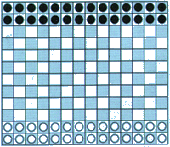
\includegraphics[scale=0.60]{epaTOP.png}
\end{center}
Os movimentos de cada peça são iguais ao do Rei do xadrez, pode andar uma casa em qualquer direção. Podem ser criados inúmeros grupos de peças, phalanxes, estas só se podem deslocar um número igual ou menor ao número de peças do grupo, na direcção da linha formada pelo grupo. Uma peça pode fazer parte de várias phalanxes. Uma phalanx pode ser dividida, mas só pode andar um número de casas igual ou menor ao numero de elementos da phalanx que se irá mover.\cite{rules}
\begin{center}
  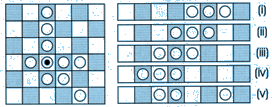
\includegraphics[scale=0.60]{epa1-2.png}
\end{center}
Não é permitido passar um jogada, em cada jogada é obrigatório mover uma phalanx ou uma peça. Todas as peças têm de estar contidas no tabuleiro. Não podem haver peças sobrepostas ou na mesma posição, exceto quando a cabeça de uma phalanx captura outra peça ou phalanx.
\begin{center}
  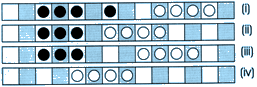
\includegraphics[scale=0.60]{epa3.png}
\end{center}
Para capturar é necessário atacar com um grupo com mais elementos que o adversário na linha de ataque. A peça/phalanx capturada é removida do tabuleiro para sempre. Um jogador ganha quando, na sua vez de jogar, tiver mais peças que o adversário na linha mais afastada de si.\cite{rules}

\section{Arquitetura do Sistema}
O jogo é iniciado com um predicado chamado start: mostra o tabuleiro inicial; lê as coordenadas através de READ\textbackslash1 e chama o predicado recursivo play(E,XS,YS,XD,YD). Este predicado faz o seguinte: na parte inicial testa os valores XS,YS,XD,YD de modo a ver se são válidos; caso sejam chama atualizarEstado(E,XS,YS,XD,YD,N); caso este objetivo seja completado, é mostrado o novo tabuleiro; são lidos os novos valores de XS,YS,XD,YD e é chamado play com os novos valores.
\\\linebreak
A função de atualizarEstado(E,XS,YS,XD,YD,N) é "corrigir" os valores de XS,YS,XD,YD visto que são mostrados de forma diferente; verificar se a jogada é válida através de canimovethere(E,XS1,YS1,XD1,YD1); se sim, mudarestado(E,XS1,YS1,XD1,YD1,N) e depois mudar a vez.
\\\linebreak
Na verificação das regras canimovethere(E,XS,YS,XD,YD): chama regras(E,XS,YS,XD,YD) e caso esta falhe é chamado badMoveFriend(E) cujo objetivo é pedir novamente que se jogue. A cláusula regras(E,XS,YS,XD,YD) contém 3 regras que verificam: se é a minha vez; se existe sobreposicao; se se pode mover uma phalanx(uma peça é um phalanx com um só elemento) ou se se pode capturar uma peça; e se estamos em condição de acabar o jogo. Se estivermos, o jogo acaba e é indicado quem ganhou.
\\\linebreak
Foram construídas várias regras úteis: getSizeTilColour('tipodelinha',); headPhalanx('tipodelinha',); checkColour(,); changechar(,)r;, findEnemyHead('tipodelinha',); movePhalanxUP(,); movePhalanxLEFT(,).Cujos objetivos são bastante óbvios.

\section{Lógica do Jogo}
\subsection{Representação do Estado do Jogo}
\begin{center}
Iremos criar um estado inicial, uma lista de listas da forma:

[[2,2,2,2,2,2,2,2,2,2,2,2,2,2],[2,2,2,2,2,2,2,2,2,2,2,2,2,2],[0,0,0,0,0,0,0,0,0,0,0,0,0,0],

  [0,0,0,0,0,0,0,0,0,0,0,0,0,0],[0,0,0,0,0,0,0,0,0,0,0,0,0,0],[0,0,0,0,0,0,0,0,0,0,0,0,0,0],

  [0,0,0,0,0,0,0,0,0,0,0,0,0,0],[0,0,0,0,0,0,0,0,0,0,0,0,0,0],[0,0,0,0,0,0,0,0,0,0,0,0,0,0],

[0,0,0,0,0,0,0,0,0,0,0,0,0,0],[1,1,1,1,1,1,1,1,1,1,1,1,1,1],[1,1,1,1,1,1,1,1,1,1,1,1,1,1]]
\end{center}
Através da regra de interface play iremos chamar as size e atualizarestado que testa as regras do jogo e atualiza o estado, caso tal respeite as regras do jogo. A regra atualizarestado chama pelas cabeças canimovethere, mudarestado e turnchange. Se a regra canimovethere não corresponder isso implica o falhanço do "if" em prolog e portanto o estado não é alterado nem a vez, sendo pedida outra vez um movimento. Se o objetivo canimovethere for bem sucedido, então podemos proceder à alteração do estado através da regra mudarestado. Restando mudar a vez do jogador, através de por exemplo de turnchange(C) (através de retract e asserta). Sendo este ciclo repetido novamente,até chegarmos a uma situação de fim de jogo.
\begin{center}
  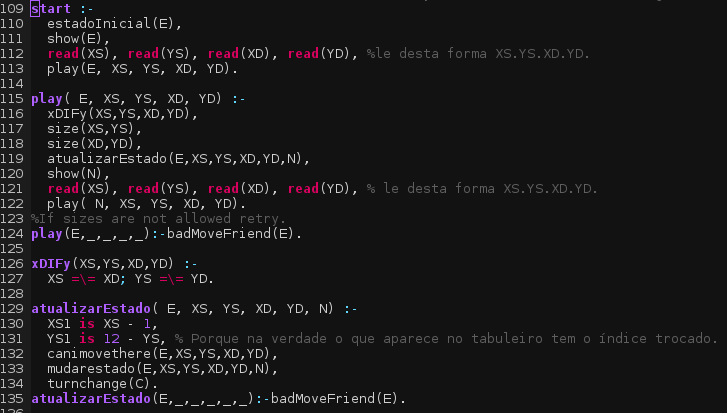
\includegraphics[scale=0.60]{representacao.png}
\end{center}
O estado vai sendo atualizado consoante as jogadas de cada jogador, o 0 significa que não há nenhuma peça nessa posição. O 1 representa uma peça branca e o 2 uma preta. Quando se imprimi o 1 passa a W e o 2 a B.
\\\linebreak
Um estado com posições intermédias,
\begin{center}
  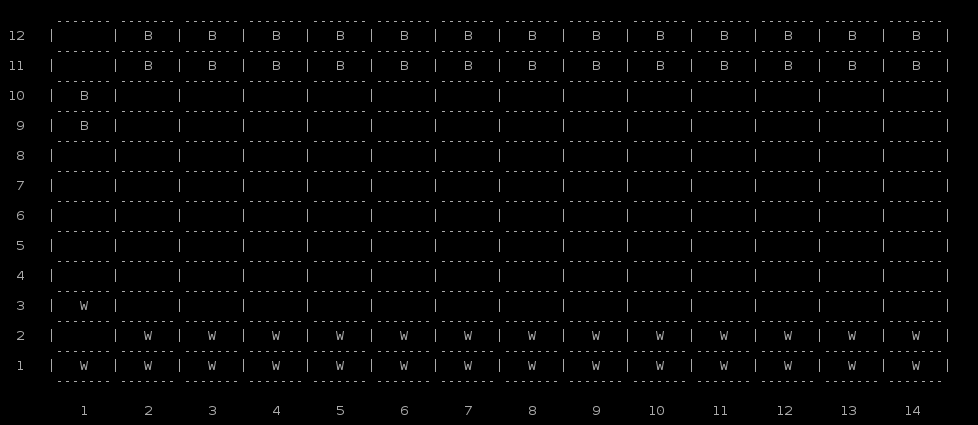
\includegraphics[scale=0.45]{intermedio.png}

[[0,2,2,2,2,2,2,2,2,2,2,2,2,2],[0,2,2,2,2,2,2,2,2,2,2,2,2,2],[2,0,0,0,0,0,0,0,0,0,0,0,0,0],

  [2,0,0,0,0,0,0,0,0,0,0,0,0,0],[0,0,0,0,0,0,0,0,0,0,0,0,0,0],[0,0,0,0,0,0,0,0,0,0,0,0,0,0],

  [0,0,0,0,0,0,0,0,0,0,0,0,0,0],[0,0,0,0,0,0,0,0,0,0,0,0,0,0],[0,0,0,0,0,0,0,0,0,0,0,0,0,0],

[1,0,0,0,0,0,0,0,0,0,0,0,0,0],[0,1,1,1,1,1,1,1,1,1,1,1,1,1],[1,1,1,1,1,1,1,1,1,1,1,1,1,1]]
\end{center}
Um estado com posições finais, qualquer configuração em que existam mais peças do adversário na minha linha mais recuada, na vez dele jogar. E vice-versa.

\subsection{Visualização do Tabuleiro}
De modo a imprimir o estado atual do tabuleiro, tem-se de construir um predicado recursivo que escreva o conteúdo de cada linha na consola e depois dê um break line. Tal pode ser feito através das seguintes cláusulas:
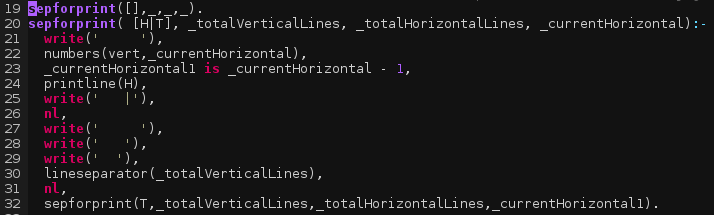
\includegraphics[scale=0.60]{imprimir.png}
\\\linebreak
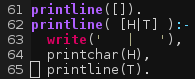
\includegraphics[scale=0.50]{imprimir1.png}
Resultando:
\\\linebreak
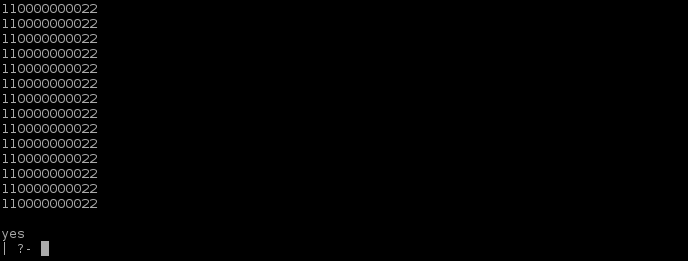
\includegraphics[scale=0.40]{tabuleiro.png}

\subsection{Validação das Jogadas}
A regra principal do nosso programa é play(E,XS,YS,XD,YD), no ínicio desta são verificados casos básicos de regras: xDIFy(XS,YS,XD,YD) verifica se as coordenadas são exatamente iguais se forem falha, size(XS,YS) vê se XS e YS estão dentro do tabuleiro e o mesmo para XD e YD. O resto das regras são verificadas em canimovethere(E,XS,YS,XD,YD), cuja cabeça está em atualizarEstado(E,XS,YS,XD,YD,N) que por sua vez está em play(E,XS,YS,XD,YD).
\\\linebreak
Em canimovethere(E,XS,YS,XD,YD) é chamado as regras(E,XS,YS,XD,YD). Lá encontram-se as regras restantes: é verificado se a cor na posição XS,YS tem o mesmo valor que a cor de quem deve jogar;

\section{Movimentos}
Cada peça pode ser movida sozinha ou em conjunto. No caso de ser só uma peça é possivel movê-la para qualquer direção, horizontal, vertical ou diagonal, em uma unidade desde que essa célula esteja vazia. No caso de se mover um conjunto de peças, estas não podem estar separadas por nenhuma célula vazia nem por peças do adversário, todas elas serão movidas até um máximo correspondente ao número de peças que se pretende mover e têm que respeitar a orientação na qual o grupo se encontra, por exemplo, se o grupo de peças se encontrar na horizontal as peças só podem ser movidas ou para a esquerda ou para a direita.
\\\linebreak
Como já foi referido iremos ter um predicado chamado canimovethere, que irá receber a peça que se pretende mover, ou no caso do conjunto de peças a peça mais recuada, e para onde queremos mover e que irá verificar se é possivel essa jogada.
\\\linebreak
Os predicados a utilizar são:
\\\linebreak
size(X,Y):- X\textgreater=1, X=\textless14, Y\textgreater=1, Y=\textless12.
\\\linebreak
play( XS, YS, XD, YD) :-  size(X,Y), atualizarEstado(XS,YS,XD,YD).
\\\linebreak
atualizarEstado( XS, YS, XD, YD) :- \textit{canimovethere(XS,YS,XD,YD)}, mudarestado(XS,YS,XD,YD),turnchange(C).

\section{Conclusões e Perspectivas de Desenvolvimento}
O Epaminondas é um jogo cheio de estratégia e regras, tivemos de fazer várias regras de remoção,testes,etc dependendo da natureza da linha de movimentação das phalanx e portanto esta parte foi, na nossa opinião, a mais trabalhosa. Infelizmente, só conseguimos acabar a parte jogador vs jogador, isto foi devido a termos outros projetos em mão. A movimentação das peças que pode ser feita em oito direções e usando só uma peça ou um conjunto de peças, no caso dos phalanxs, sempre tendo em atenção os limites do tabuleiro e as outras peças, quer sejam do próprio jogador o que impossibilita a jogada ou do jogador adversário cujas peças têm de ser removidas do tabuleiro, no caso de ter menos peças no phalanx, ou então serão as peças do próprio a serem removidas, irá ser a parte mais desafiante a implementar.
\\\linebreak
Gostaríamos de ter acaba o trabalho em tempo útil mas não nos foi possível. Mas na globalidade foi uma boa experiência aprender a pensar em PROLOG.
\\\linebreak

\clearpage
\addcontentsline{toc}{section}{Bibliografia}
\renewcommand\refname{Bibliografia}
\bibliographystyle{plain}
\bibliography{myrefs}

\end{document}
